\subsection{Ideation, formulation and analysis.}

To make a quadrature oscillator, we must first create an oscillator that would provide a sinusoidal wave and then create a device that would phase shift the signal by 90$^\circ$. We then adjust the other parameters to model our two waves.

For the sinusoidal wave oscillator, we are using a Wien- bridge oscillator (as shown in \Cref{fig:wien_bridge})`. The Wien bridge oscillator is a type of electronic oscillator that generates sinusoidal waves without any external input signal. It uses a combination of positive and negative feedback networks. It is a good oscillator to generate low distortion sinusoidal signals.

\begin{figure}[h]
    \centering
    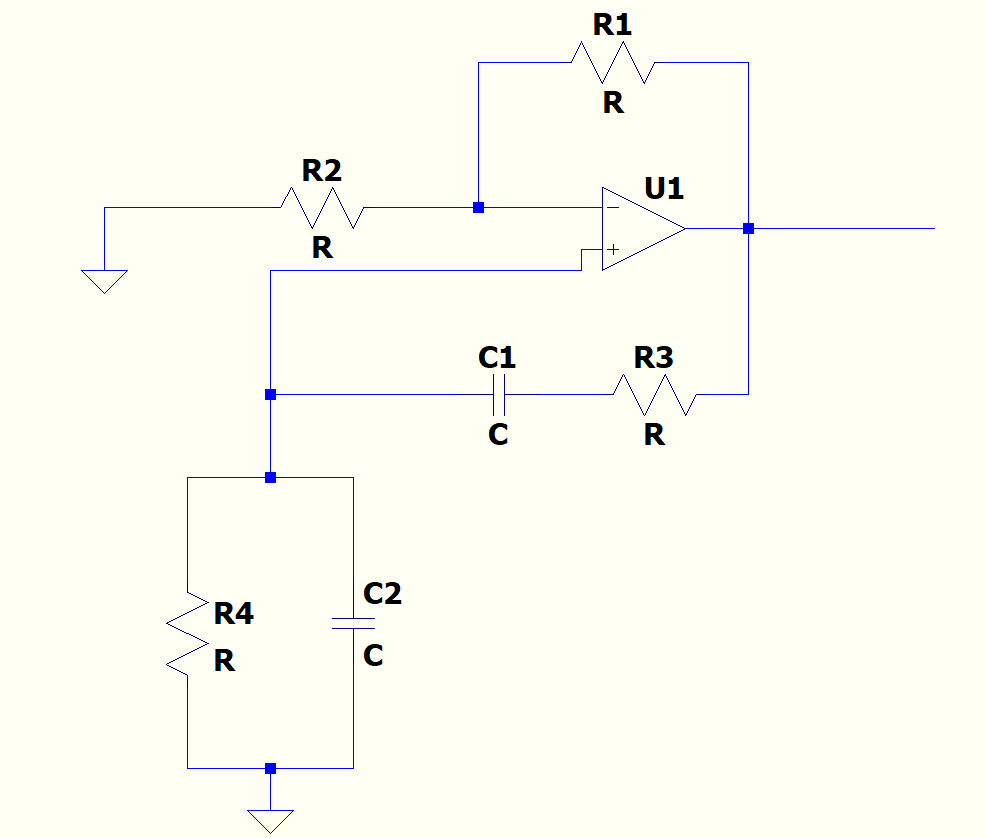
\includegraphics[width=0.6\linewidth]{fig/wien-bridge-schem.png}
    \caption{Wien Bridge Oscillator}
    \label{fig:wien_bridge}
\end{figure}




The positive feedback network is responsible for the resonant frequency setup and oscillation whereas the negative feedback network is responsible for the amplification.

In the positive feedback network, two RC networks one in series and the other in parallel are connected in series in the positive feedback network. The two RC networks are a low pass filter and a high pass filter which collectively acts as a notch pass filter so only a certain frequency is passed through it (Resonance Frequency).

In \Cref{fig:wien_bridge}, we take
\[
  R_3 = R_4 = R, \quad C_1 = C_2 = C
\]
Calculating the impedance of the circuit components,
$$Z_{R3} = Z_{R4} = R$$
$$Z_{C1} = Z_{C2} = \frac{1}{sC}$$

Resistor and capacitor connected in series forms the High Pass Filter,
$$Z_{HPF} = R + \frac{1}{sC}$$

Resistor and capacitor connected in parallel forms the low pass filter.
$$Z_{LPF} = \frac{1}{\frac{1}{R} + sC}$$

Voltage divider at non inverting input
$$V_+ = \frac{Z_{LPF}}{Z_{LPF} + Z_{HPF}} V_{out}$$
$$V_+ = \frac{\frac{1}{\frac{1}{R} + sC}}{R + \frac{1}{sC} + \frac{1}{\frac{1}{R} + sC}} V_{out}$$
simplifies into
$$V_+ = \frac{R}{R + \frac{(1 + sRC)^2}{sC}} V_{out}$$


 $$s = j \omega $$
$$\therefore V_+ = \frac{R}{R + \frac{(1 + j \omega RC)^2}{j \omega C}} V_{out}$$

\begin{equation}
\boxed{V_+ = \frac{R}{R + \frac{(1 + j \omega RC)^2}{j \omega C}} V_{out}}
\label{eqn. 1}
\end{equation}


For the negative feedback network,
\begin{equation}
    \boxed{V_{out} = (1 + \frac{R_1}{R_2})V_+}
    \label{eqn. 2}
\end{equation}

using \cref{eqn. 1} and \cref{eqn. 2},

$$V_{\text{out}} = \left(1 + \frac{R_1}{R_5}\right) V_+ 
= (1 + \frac{R_1}{R_2}) \frac{R}{R + \frac{(1 + j\omega R C)^2}{jC\omega}} V_{out}$$

$$\implies 1 = (1 + \frac{R_1}{R_2})\frac{R}{R + \frac{(1 + j\omega R C)^2}{jC\omega}}$$

for $\frac{(1 + j\omega R C)^2}{jC\omega}$ to be real,

$$\angle(jC\omega) = 90^\circ$$
$\therefore$ we want the numerator also to be in $90^\circ$
$$\implies \angle(1 + jRC\omega)^2 = 90^\circ$$
$$\implies Re\{(1 + jCR\omega )\} = Im\{(1 + jCR\omega)\}$$
$$\implies 1 = CR\omega$$
$$\therefore \omega = \frac{1}{RC}$$
\begin{equation}
    \omega = \frac{1}{RC}
    \label{eqn.3}
\end{equation}

therefore, the resonant frequency becomes,
$$\boxed{f_r = \frac{1}{2\pi R C}}$$
from \cref{eqn.3},\\
\\
 \[
\text{Loop gain}= \left(1 + \frac{R_1}{R_2} \right) \cdot \frac{R}{R + R\frac{(1 + j)^2}{j}}
\]
$$\implies \text{Loop Gain} = {\left(1 + \frac{R_1}{R_2}\right)}\frac{1}{1 + \frac{2j}{j}}$$
$$\implies \text{Loop gain} = \left(1 + \frac{R_1}{R_2}\right)\frac{1}{3}$$
\\
To sustain oscillations, Loop gain = 1
$$\boxed{\therefore \frac{R_1}{R_2} = 2}$$

The Amplitude of the oscillations is determined by the dynamically regulated non linear feedback mechanism that adjusts the gain to maintain steady oscillations.

We are tasked to make a quadrature oscillator that produces a sine wave of frequency of 100 KHz and amplitude of $1V_{pp}$. The sine wave should oscillate between $+0.5V_{pp}$ and $-0.5V_{pp}$.\\

Selecting a standard value for $C = 1 \text{nF}$\\
so, $R$ should be $R \approx 1.59\text{ K}\Omega$

For $ R = 1.6 \text{K}\Omega$ and $C = 1\text{nF}$, $f_r \approx 100\text{KHz}$.

And $\frac{R_1}{R_2} = 2$, so we take $R_1 = 20 K\Omega$ and $R_2 = 10 K\Omega$.\\
\\
Theoretical values are calculated.\\
When put these values to simulation, the frequency of the oscillation was approx. 50KHz, which is half the frequency we need. After fine tuning the components to arrive at a frequency of $100KHz$, the components take up the following values:

$$R = 900\Omega$$
$$C = 0.9nF$$
$$R_1 = 25K\Omega$$
$$R_2 = 10K\Omega$$

This gives the oscillation of frequency 100KHz and amplitude 710 mV. To adjust the amplitude to 500mV, we use a voltage divider to control it.

\begin{figure}[H]
    \centering
    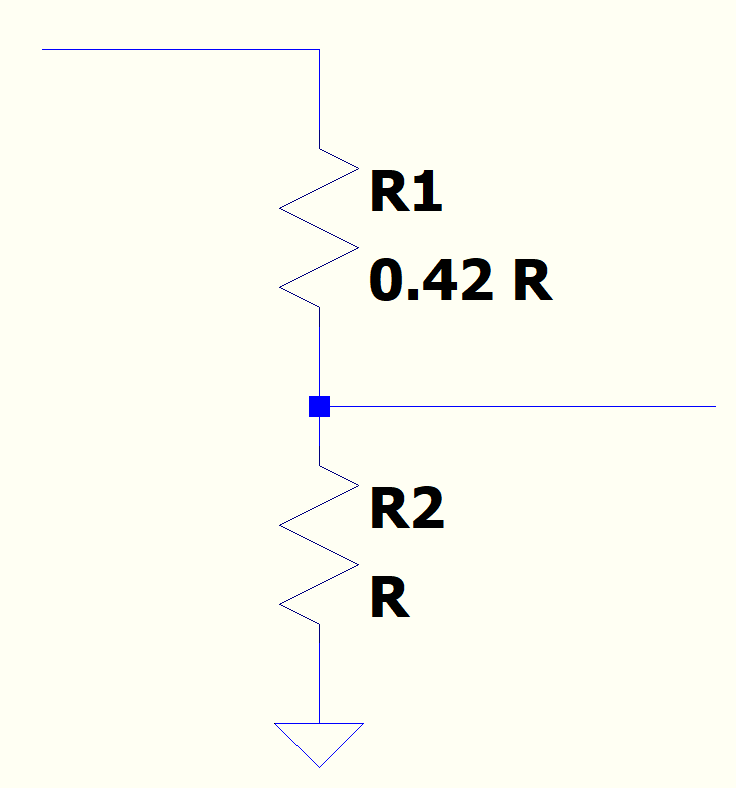
\includegraphics[width=0.6\linewidth]{Voltage-divider.png}
    \caption{Voltage Divider}
    \label{fig:voltage-div}
\end{figure}

In the Voltage divider,
$$V_{out} = V_{in}\cdot \frac{R_2}{R_1 + R_2}$$
$$\implies 500\text{ mV} = 710 \text{ mV} \cdot \frac{R_2}{R_1 + R_2}$$
$$\implies 0.704 = \frac{R_2}{R_1 + R_2}$$
$$\implies \frac{R_1}{R_2} = \frac{1}{0.704} - 1 \approx 0.42$$

Taking standard values, $R_2 = 10K\Omega$ and $R_1 = 4.2K\Omega$.
In the simulation, we got a value of 524 mV from the voltage divider. After fine tuning the values to achieve 500 mV, the values arrived at are,
$$R_1 = 5.1K\Omega$$
$$R_2 = 10k\Omega$$

We take one output from this voltage divider, this will be our In-phase component of the quadrature oscillator.\\
We take this signal to phase shift it by $90^\circ$, 

\begin{figure}[H]
    \centering
    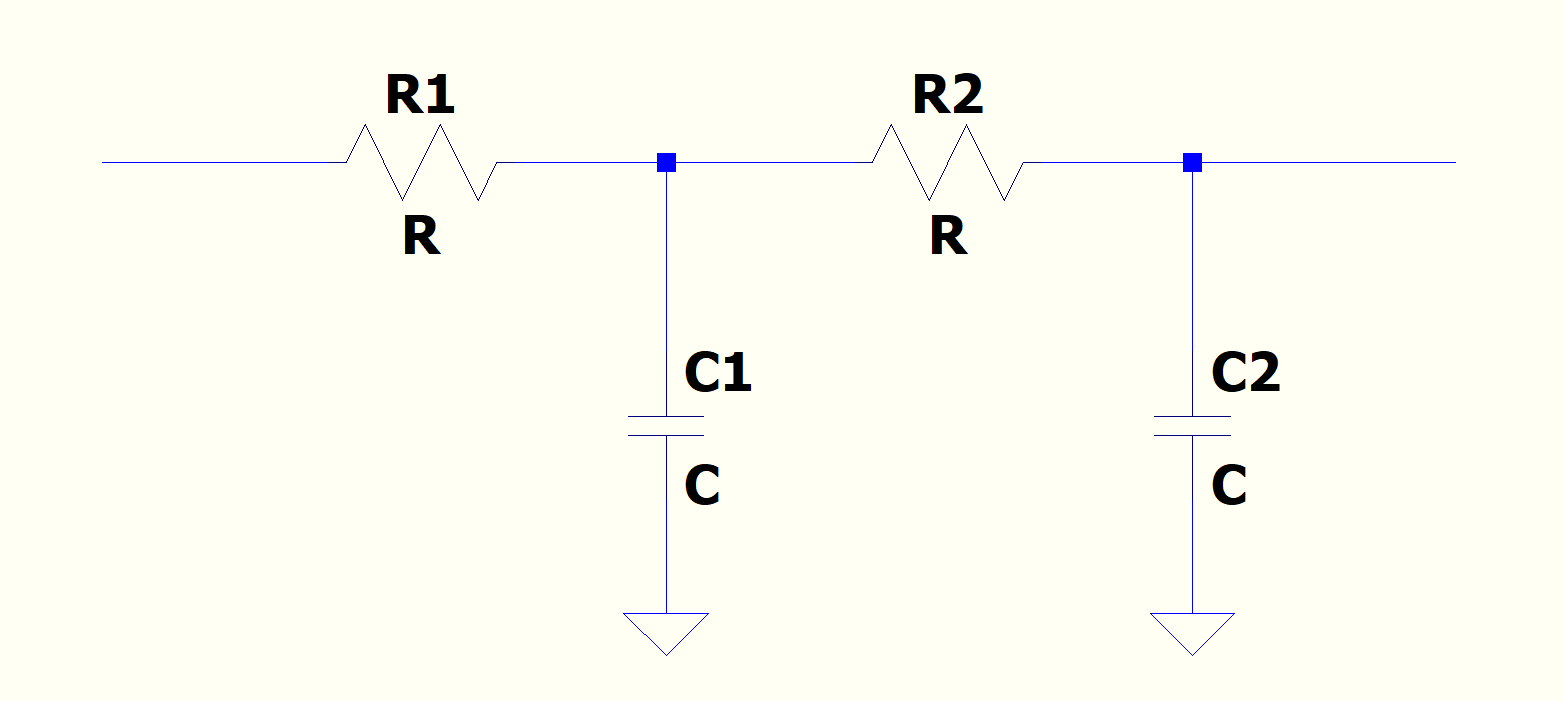
\includegraphics[width=0.8\linewidth]{Phase-shift.png}
    \caption{Phase Shifter}
    \label{fig:phase-shift}
\end{figure}

There are 2 RC stages in this circuit block (refer to \cref{fig:phase-shift}). Each RC stage provides a phase shift of $45^\circ$ which gives a total phase shift of $90^\circ$.
\\
\\
For each RC stage, transfer function of the stage is
$$H(\omega) = \frac{1}{ 1 + j\omega RC}$$\\
The phase shift of this stage is 
$$\phi(\omega) = -\tan^{-1}(\omega RC)$$
This is a lagging phase shift, for two stages
$$\phi_{tota} = 2 \cdot \phi = -90^\circ \implies \phi = -45^\circ \text{ per stage}$$
To solve for RC at $45^\circ$
$$\tan^{-1}(\omega RC) = \frac{\pi}{4} \implies \omega RC = \tan(\frac{\pi}{4}) = 1$$
we substitute, $\omega = 2\pi f = 2\pi \cdot 10^5 rad/s$
$$RC = \frac{1}{\omega} = \frac{1}{2\pi \cdot 10^5} = 1.595 \times 10^{-6}s$$
For standard values,
$$R = 1.6K\Omega$$
$$C = 1nF$$

When simulated with the theoretical values, the time difference between two peaks of the two waves comes out to be $2.2 \mu s$ which give the phase shift by approximately $-109^\circ$. After fine tuning the values, for phase shift by $-90^\circ$, the time difference between the two wave peaks should be equal to $2.5 \mu s$.
$$T = \frac{1}{f} \text{(Period of the wave)}$$
Phase shift by $90^\circ$ means $\Delta t = \frac{T}{4}$
$$\implies T = \frac{1}{100000} = 10 \mu s$$
$$\implies \Delta t = \frac{10 \mu s}{4} = 2.5 \mu s$$

The values of the components after fine tuning comes as,
$$R = 1K\Omega$$
$$C = 0.93nF$$

This also attenuates the amplitude of the wave to 256 mV.
To maintain the amplitude of the phase shifted wave at 500 mV, we use an op-amp amplifier to do the same.
\begin{figure}[H]
    \centering
    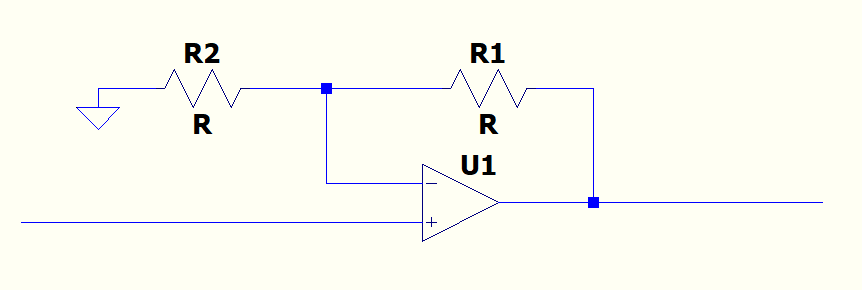
\includegraphics[width=0.75\linewidth]{op-amp-amplifier.png}
    \caption{Op-amp inverting Amplifier}
    \label{fig:op-amp-amp}
\end{figure}

$\because$ the phase shift from the RC Phase shift circuit is $-90^\circ$, we can use an inverting amplifier so that the total phase shift becomes $180^\circ - 90^\circ = 90^\circ$.

This converts the lagging phase shift into leading phase shift.\\
\\
We know,

$$\text{Gain } = \frac{V_{out}}{V_{in}} = \frac{500mV}{256mV} \approx 1.95$$

$\because$ the circuit is an inverting amplifier, we know
$$A_v = -\frac{R_1}{R_2}$$
as we are inverting the signal, we ignore the negative sign for calculations.

$$1.95 = \frac{R_1}{R_2}$$
Taking standard value for $R_2 = 10K\Omega$, we get $R_1 = 40.65K\Omega$
$$R_1 = 19.53K\Omega$$
$$R_2 = 10K\Omega$$

When simulated with the theoretical values, the amplitude of the phase shifted wave was approx. 760m V. When fine tuned the component values for amplitude 500 mV, we get the following values,
$$R_1 = 8.4K\Omega$$
$$R_2 = 8.9K\Omega$$

Now, we have the amplitude of the phase shifted wave is 500 mV. The output of this inverting amplifier, is our quadrature component of the oscillator.\\
\\
To make sure that none of the impedance of the different circuit blocks affect the achieved signal, we use a voltage buffer between the circuit blocks (\cref{fig:op-amp-buffer}).
\begin{figure}[H]
    \centering
    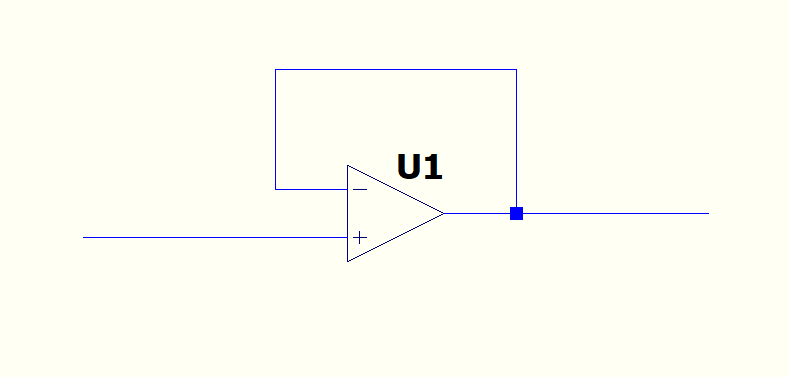
\includegraphics[width=1\linewidth]{voltage-buffer.png}
    \caption{Op-amp Voltage Buffer}
    \label{fig:op-amp-buffer}
\end{figure}
We are now done with the design of our quadrature oscillator.

\begin{figure}[H]
    \centering
    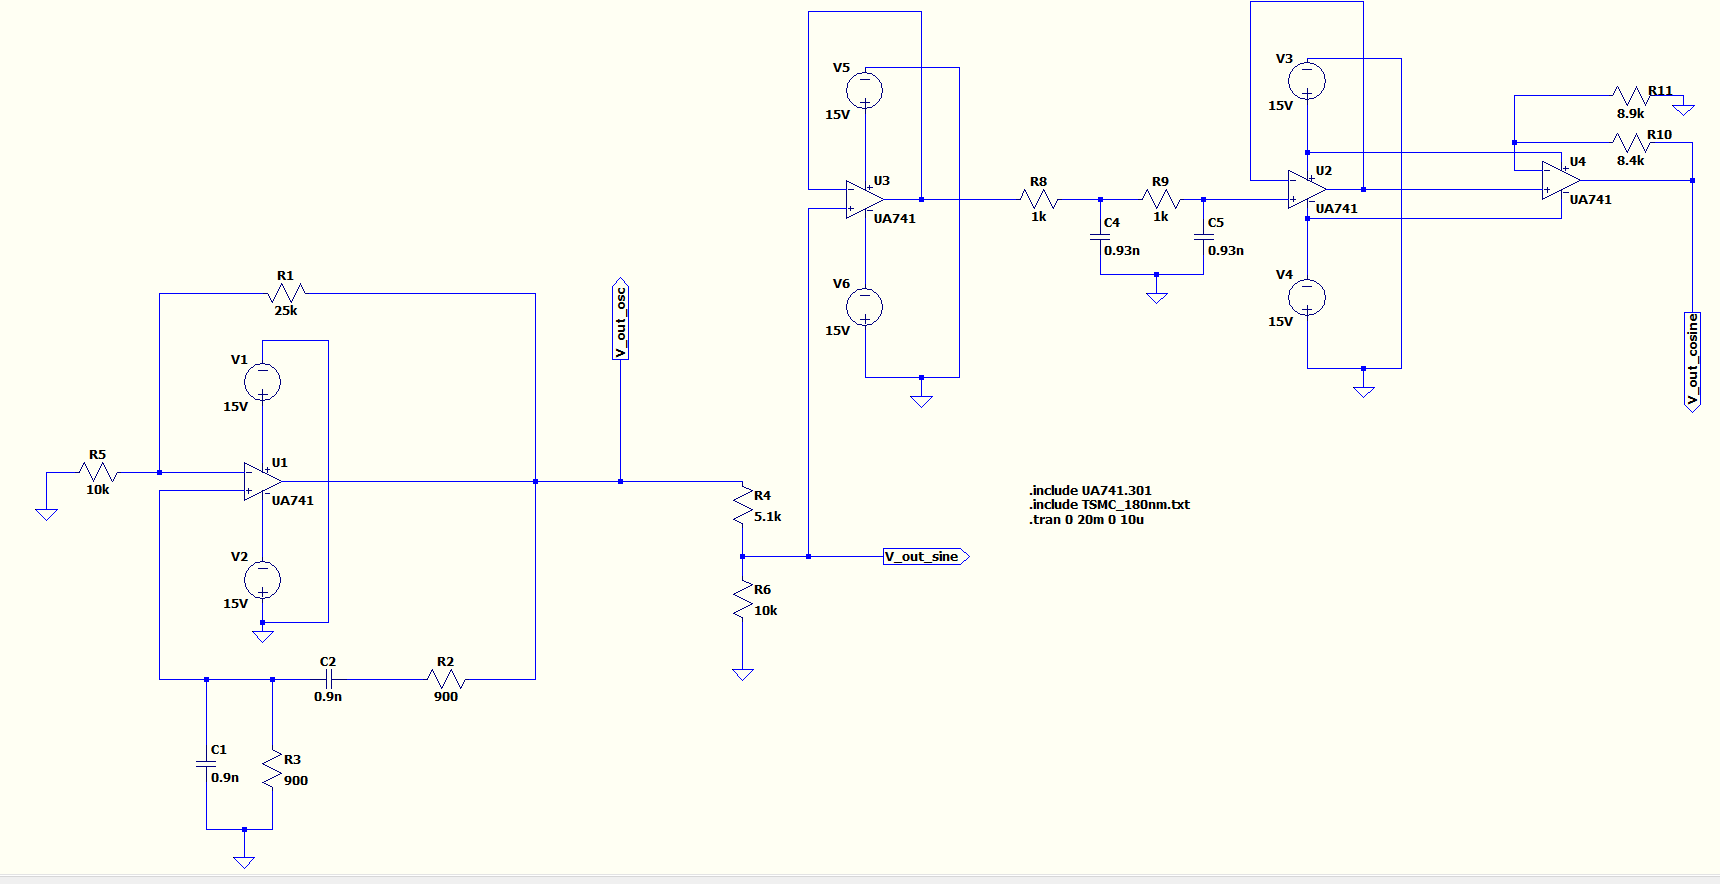
\includegraphics[width=1\linewidth]{quad-osc-ckt.png}
    \caption{Quadrature Oscillator Circuit}
    \label{fig:enter-label}
\end{figure}

\subsection{Simulation and results.}
\begin{figure}[H]
    \centering
    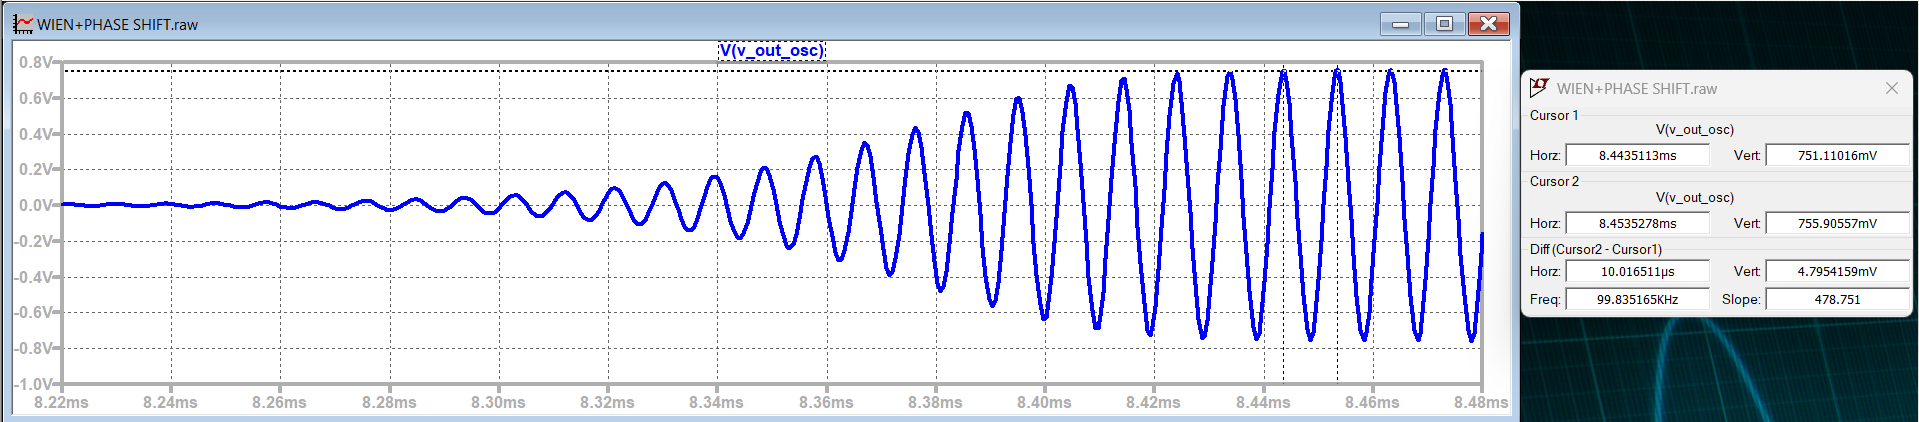
\includegraphics[width=1\linewidth]{wien-osc-output.png}
    \caption{Output signal of the Wien-bridge oscillator}
    \label{fig: wien-output}
\end{figure}

Frequency of the wave is $\approx 100 KHz$ and amplitude is $\approx 750mV$.\\
To adjust the amplitude, we used a voltage divider.
\begin{figure}[H]
    \centering
    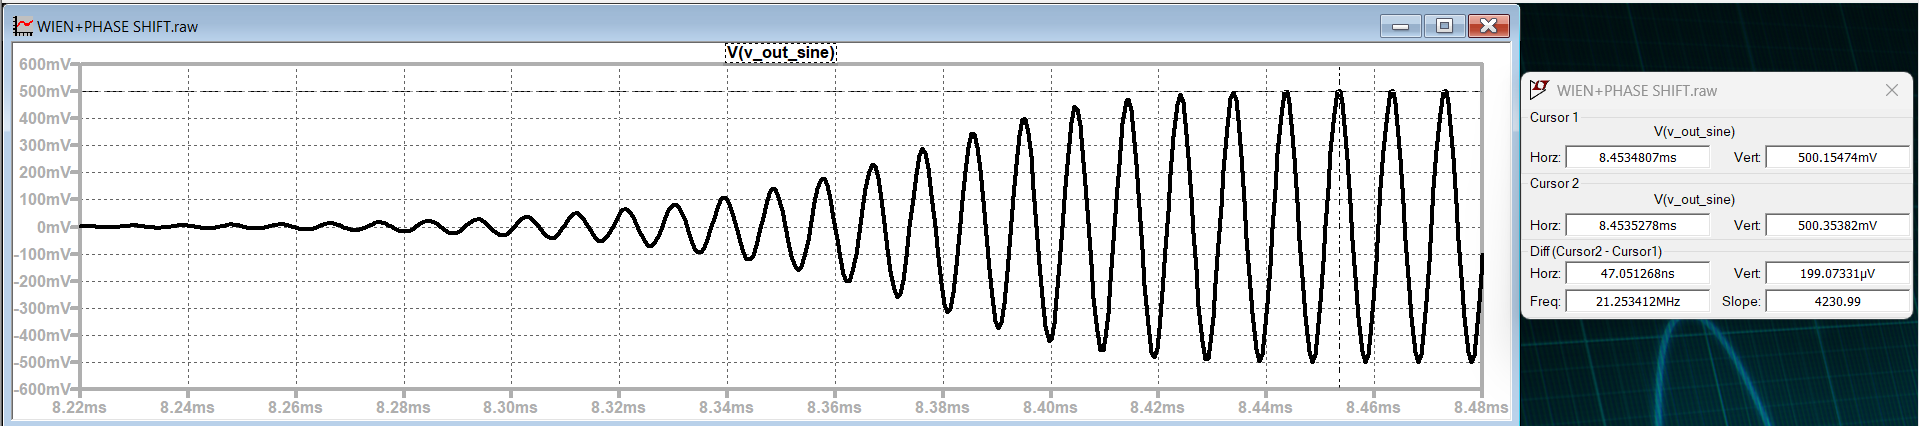
\includegraphics[width=1\linewidth]{voltage-div-output.png}
    \caption{Output signal of the voltage divider.}
    \label{fig:enter-label}
\end{figure}

Amplitude of the sine wave is now set at 500 mV, this is our in-phase component of the signal. For quadrature component, we phase shifted it using the RC Phase shift circuit.
\begin{figure}[H]
    \centering
    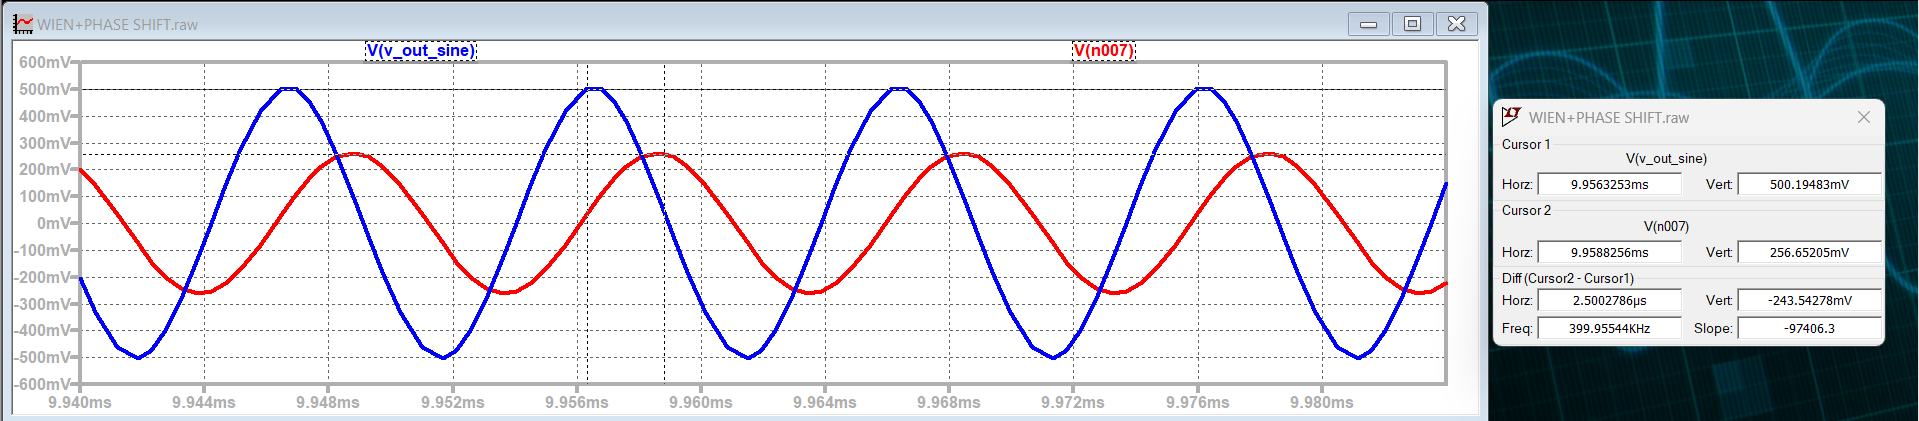
\includegraphics[width=1\linewidth]{RC-phase-shift-output.png}
    \caption{Output signal of the RC Phase shift circuit}
    \label{fig:rc-phase-shift-output}
\end{figure}
As you can see the time difference between the two peaks of the waves is $2.5 \mu s$ which is what we calculated earlier. The wave is phase shifted by $90^\circ$.\\
We used an inverting op-amp amplifier to maintain the amplitude of the quadrature component at 500 mV.
\begin{figure}[H]
    \centering
    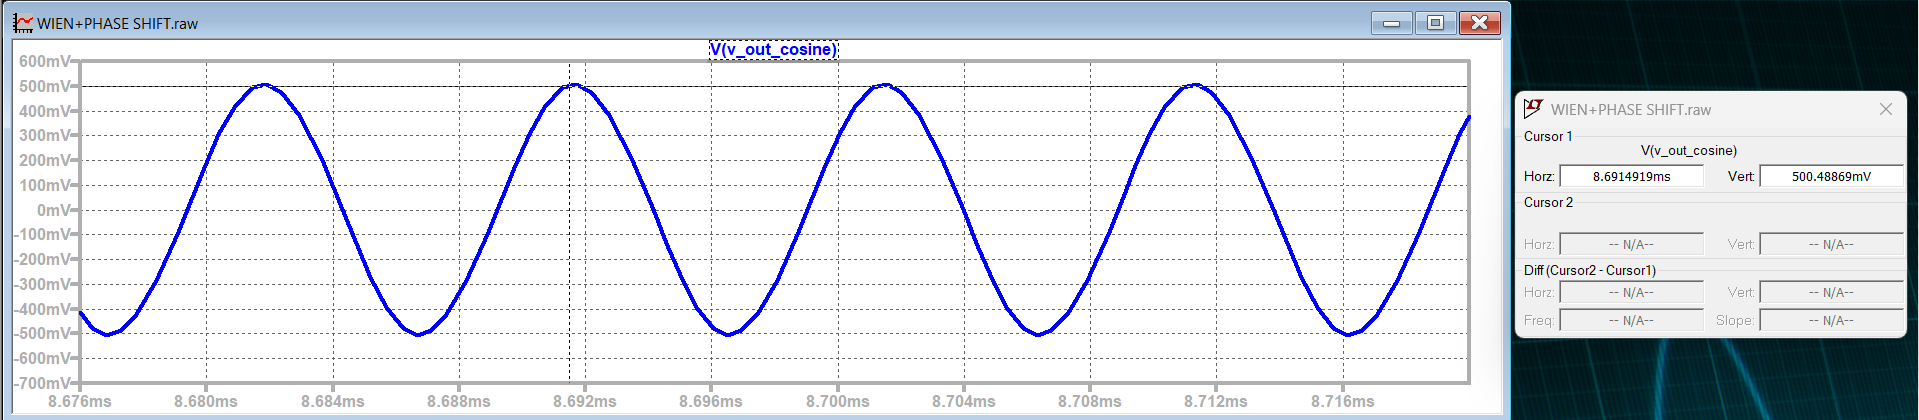
\includegraphics[width=1\linewidth]{op-amp-amp-output.png}
    \caption{Output signal of the Inverting op-amp amplifier}
    \label{fig:enter-label}
\end{figure}

This is our quadrature component of the oscillator.\\
\\
The final result of the simulation is as follows:
\begin{figure}[H]
    \centering
    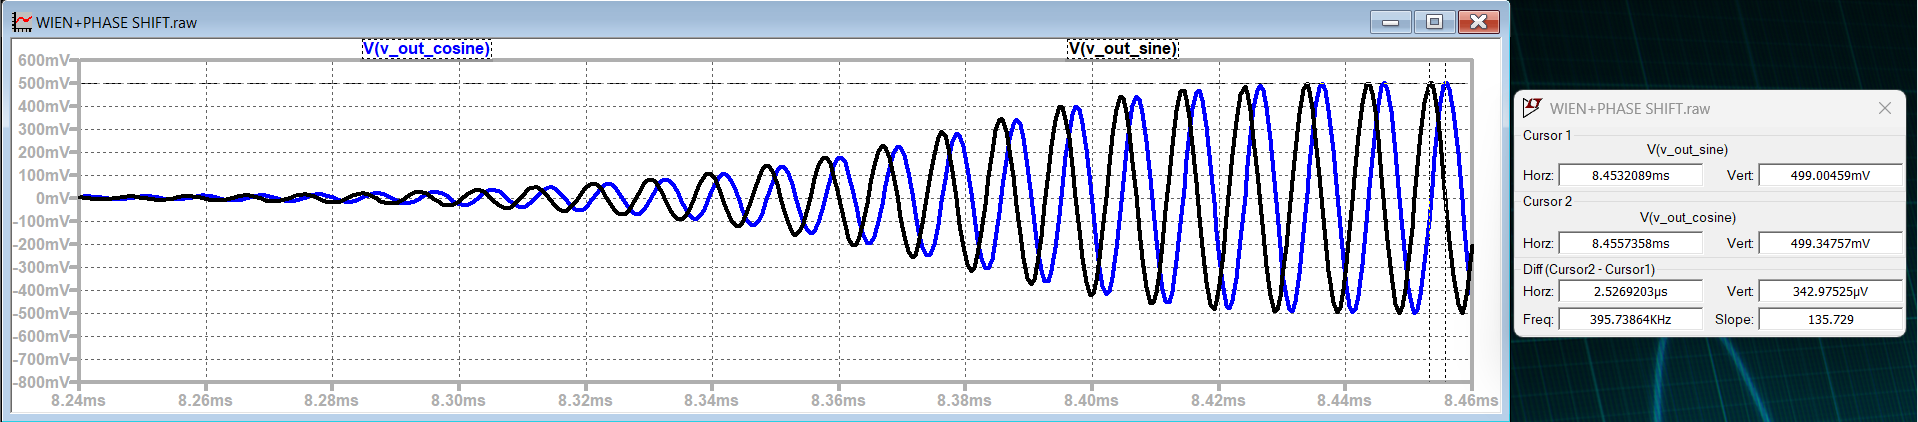
\includegraphics[width=1\linewidth]{Final-simulation-result.png}
    \caption{Final simulation Result}
    \label{fig:enter-label}
\end{figure}

As shown in the result the amplitude of the in-phase component of the signal (V\_out\_sine) and quadrature component of the signal (V\_out\_cosine) is $\approx 500 mV$ and the time difference between two simultaneous peaks of the wave is $\approx 2.5 \mu s$, which concludes that the phase difference between the two waves is $90^\circ$.\\
\\
This is our desired quadrature oscillator.